% Include Preamble 
\documentclass[10pt,dvipsnames, aspectratio=169]{beamer}
\usetheme[progressbar=frametitle]{metropolis}
\usepackage[]{verbatim}\usepackage[]{}
\usepackage{booktabs}
\usepackage[misc]{ifsym}
\usepackage{wasysym}
\usepackage{listings}
\usepackage{xspace}
\usepackage{tikz}
\newcommand{\source}[1]{\caption*{Source: {#1}} }

\usepackage{amsmath}
\usepackage{dirtytalk}
\usepackage{caption}
\usepackage{subcaption}
\usepackage{xcolor}
\usepackage{ragged2e}\justifying % for justify content % Customize 
\setlength{\parskip}{5pt} % vertical spacing between 2 paragraphs
\setbeamersize{text margin left=12mm, text margin right=12mm} 
\setbeamertemplate{frametitle}[default][left, leftskip=8mm]
%\usepackage[hidelink]{hyperref}
\newcommand{\themename}{\textbf{\textsc{metropolis}}\xspace}

% WARNING: Don't Touch,if you are not compfortable! 
\addtobeamertemplate{frametitle}{}{
%\begin{tikzpicture}[remember picture,overlay]
%\node[anchor=north east,yshift=2pt,xshift=-65pt] at (current page.north east) 
%{\includegraphics[height=.75cm]{img/elixir-portugal-white}};
%\node[anchor=north east,yshift=4pt] at (current page.north east) 
%{
\includegraphics[height=1cm]{img/hdro}};
%\end{tikzpicture}
}

% Title Page of Presentation 
% WARNING: Don't change logo, just write your details 
\title{ISCB20.05--Introduction to Biostatistics}
\date{\today}
\author{Md. Jubayer Hossain\\
        https://jhossain.me/}
\institute{Lead Organizer, Introduction to Scientific Computing for Biologists 
\\ Founder, Health Data Research Organization}
\titlegraphic{\vspace{4cm}\hfill
\includegraphics[height=1cm]{img/hdro2}}
\begin{document}
\maketitle
% Sectuion Title 
\section{Section-1.2: Data Research Methods}
% Slide-Overview
\begin{frame}[t]{Overview}
	\begin{itemize}
		\item What is Research? Research Process
		\item Types of Research 
		\item Sampling and Sampling Methods
		\item Data Collection Methods 
		\item Types of Statistical Methods
		\item Steps in a Research Project
	\end{itemize}
\end{frame}
% slide-1 
\begin{frame}[t]{What is Research?}
	\textbf{Definition-1} \\ 
	Research is "creative and systematic work undertaken to increase the stock 
	of knowledge". It involves the collection, organization, and analysis of 
	information to increase understanding of a topic or issue. A research 
	project may be an expansion on past work in the field.
	(\url{https://en.wikipedia.org/wiki/Research})
	
	\textbf{Definition-2} \\ 
	Research is defined as the creation of new knowledge and/or the use of 
	existing knowledge in a new and creative way so as to generate new 
	concepts, methodologies and understandings. This could include synthesis 
	and analysis of previous research to the extent that it leads to new and 
	creative outcomes.
	(\url{https://www.westernsydney.edu.au/research/researchers/})
	
	\textbf{Definition-3} \\
	Simply, Research is an organized and systematic way of finding answers to 
	questions.
\end{frame}
% Slide-1
\begin{frame}[t]{Research Process}
	\begin{figure} [ht]
		\centering
		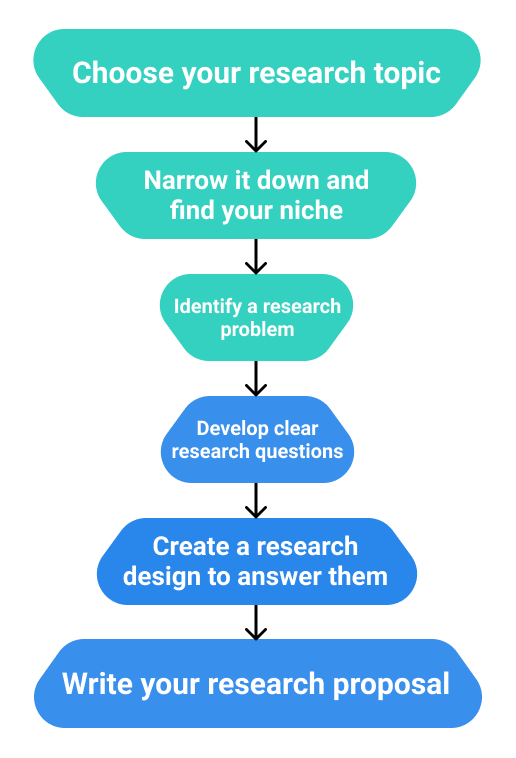
\includegraphics[width=0.3\textwidth]{rp/rp.png}
		\source{\url{https://www.scribbr.com/category/research-process/}}
	\end{figure}
\end{frame}


% Slide-2
\begin{frame}[t]{Types of Research--1}
\textbf{Application}
\begin{itemize}
	\item \textbf{Fundamental Research}: Basic research aims to develop 
	knowledge, 
	theories and predictions
	\item \textbf{Applied Research:} Applied research aims to develop 
	techniques, products and procedures.
\end{itemize}
\end{frame}

% Slide-2
\begin{frame}[t]{Types of Research--2}
	\textbf{Objective}
	\begin{itemize}
		\item \textbf{Exploratory}:  Exploratory research aims to explore the 
		main 
		aspects of under-researched problem.
		\item \textbf{Explanatory:} Explanatory research aims to explain the 
		causes 
		and consequences of a well-defined problem.
		
		\item \textbf{Descriptive:} Descriptive research aims to accurately and 
		systematically 
		describe a population, situation or phenomenon.
		
		\item \textbf{Correlational:} Correlational research is a type of 
		research 
		method that involves 
		observing two variables in order to establish a statistically 
		corresponding relationship between them.
	\end{itemize}
\end{frame}

% Slide-3
\begin{frame}[t]{Types of Research--3}
	\textbf{Inquiry Mode}
	\begin{itemize}
		\item \textbf{Quantitative:} Quantitative research is expressed in 
		numbers and graphs.
		\item \textbf{Qualitative:} Qualitative research is expressed in words.
	\end{itemize}
\end{frame}



% Slide-RM-1
\begin{frame}[t]{Fundamental or Basic Research}
	\begin{itemize}
		\item Investigation on basic principles and reasons for occurrences of 
		a particular event or process or phenomenon.
		\item It is also called theoretical research.
		\item Some natural phenomenon or relating to pure science
		\item Basic researches sometimes may not lead to immediate use or 
		application.
		\item It helps to build new frontiers of knowledge 
		\item Outcomes of basic research from the basis for many applied 
		research.
	\end{itemize}
\textbf{Examples}
\begin{itemize}
	\item An investigation into the secondary symptoms of the Human Papilloma 
	Virus (HPV). 
	\item An investigation into the symptoms of diarrhea. 
\end{itemize}
\end{frame}

% Slide-RM-2
\begin{frame}[t]{Applied Research}
	\begin{itemize}
		\item Solve certain problems employing well known and accepted theories 
		and principles.
		\item Most of the experimental research, case studies and 
		inter-disciplinary research essentially applied research.
		\item Studies individuals or specific cases without the objective to 
		generalize.
		\item Tries to say how things can be changed 
		\item Tries to correct facts which are problematic.
	\end{itemize}

\textbf{Examples}
\begin{itemize}
	\item An investigation to determine the healing properties of mushrooms.
	\item An investigation to determine the side effects of alcohol 
	consumption. 
\end{itemize}
\end{frame}



%Slide-RM-3
\begin{frame}[t]{Exploratory Research}
	\begin{itemize}
		\item Exploratory research aims to explore the main aspects of 
		under-researched problem.
		\item Exploratory type of research is usually conducted to have a 
		better understanding of the existing problem, but usually doesn't lead 
		to a conclusive result. 
	\end{itemize}
\end{frame}


% Slide-RM-4 
\begin{frame}[t]{Explanatory Research}
	\begin{itemize}
		\item Explanatory research aims to explain the causes and consequences 
		of a well-defined problem.
		\item Explanatory research is also known as causal research 
		\item Explanatory research is conducted in order to identify the extent 
		and nature of cause-and-effect relationships.
		\item  Causal research can be conducted in order to assess impacts of 
		specific changes on existing norms, various processes etc.
		\item Causal studies focus on an analysis of a situation or a specific 
		problem to explain the patterns of relationships between variables. 
	\end{itemize}
\end{frame}



%RM-5
\begin{frame}[t]{Descriptive Research}
	\begin{itemize}
		\item Descriptive research aims to accurately and systematically 
		describe a population, situation or phenomenon. It can answer what, 
		where, when and how questions, but not why questions.
		\item A descriptive research design can use a wide variety of research 
		methods to investigate one or more variables. 
	\end{itemize}
\end{frame}


\begin{frame}[t]{Correlational Research}
	\begin{itemize}
		\item Correlational research is a type of research method that involves 
		observing two variables in order to establish a statistically 
		corresponding relationship between them.
		\item The aim of correlational research is to identify variables that 
		have some sort of relationship do the extent that a change in one 
		creates some change in the other. 
	\end{itemize}
\end{frame}


% Slide-n
\begin{frame}[t]{Quantitative Research}
	\begin{itemize}
		\item Focuses on testing theories and hypotheses	
		\item Analyzed through math and statistical analysis	
		\item Mainly expressed in numbers, graphs and tables
		\item Requires many respondents	
		\item Closed (multiple choice) questions	
		\item Key terms: testing, measurement, objectivity, replicability
	\end{itemize}
\end{frame}



% Slide-n
\begin{frame}[t]{Qualitative Research}
	\begin{itemize}
		\item Focuses on exploring ideas and formulating a theory or hypothesis
		\item Analyzed by summarizing, categorizing and interpreting
		\item Mainly expressed in words
		\item Requires few respondents
		\item Open-ended questions
		\item Key terms: understanding, context, complexity, subjectivity
	\end{itemize}
\end{frame}

% Slide-n
\begin{frame}[t]{Types of Study Design}
	\begin{itemize}
		\item \textbf{Observational:} A study where a researcher records or 
		observes the observations or measurements without manipulating any 
		variables. These studies show that there may be a relationship but not 
		necessarily a cause and effect relationship. 
		\item \textbf{Experimental:} A study that involves some random 
		assignment* of a treatment; researchers can draw cause and effect (or 
		causal) conclusions. An experimental study may also be called a 
		scientific study or an experiment.
	\end{itemize}
\centering 
(Source: \url{https://online.stat.psu.edu/stat800/lesson/3/3.4})
\end{frame}

% Slide-n
\begin{frame}[t]{Problem 1: Drinking Tea before Bedtime}
	A study took random sample of adults and asked them about their bedtime 
	habits. The data showed that people who drank a cup of tea before bedtime 
	were more likely to go to sleep earlier than those who didn't drink tea.
	\begin{itemize}
		\item Observational(Correct Answer)
		\item Experimental
	\end{itemize}
\centering
(Source: \url{https://www.khanacademy.org/math/ap-statistics/})
\end{frame}

\begin{frame}[t]{Problem 2: Drinking Tea before Bedtime}
	Another study took a group of adults and randomly divided them into two 
	groups. One group was told to drink tea every night for a week, while the 
	other group was told not to drink tea that week. Researchers then compared 
	when each group fell asleep.
	\begin{itemize}
		\item Observational
		\item Experimental(Correct Answer)
	\end{itemize}
\centering
(Source: \url{https://www.khanacademy.org/math/ap-statistics/})
\end{frame}

% Slide-n
\begin{frame}[t]{Cross-sectional Study}
	\begin{itemize}
		\item A cross-sectional study is a type of research design in which you 
		collect data from many different individuals at a single point in time. 
		In cross-sectional research, you observe variables without influencing 
		them.
		\item Researchers in economics, psychology, medicine, epidemiology, and 
		the other social sciences all make use of cross-sectional studies in 
		their work.
		
	
	\end{itemize}
\textbf{When to Use?}
\begin{itemize}
	\item When you want to examine the prevalence of some outcome at a 
	certain moment in time, a cross-sectional study is the best choice.
\end{itemize}
\end{frame}


% Slide-n
\begin{frame}[t]{Case Study}
	\begin{itemize}
		\item A case study is a detailed study of a specific subject, such as a 
		person, group, place, event, organization, or phenomenon. Case studies 
		are commonly used in social, educational, clinical, and business 
		research.
		\item A case study research design usually involves qualitative 
		methods, but quantitative methods are sometimes also used. 
		\item Case studies are good for describing, comparing, evaluating and 
		understanding different aspects of a research problem.
	
	\end{itemize}
\textbf{When to Use?}
\begin{itemize}

	\item A case study is an appropriate research design when you want to gain 
	concrete, contextual, in-depth knowledge about a specific real-world 
	subject. It allows you to explore the key characteristics, meanings, and 
	implications of the case.
\end{itemize}
\end{frame}


% Slide-n
\begin{frame}[t]{Sampling}
	\begin{figure} [ht]
		\centering
		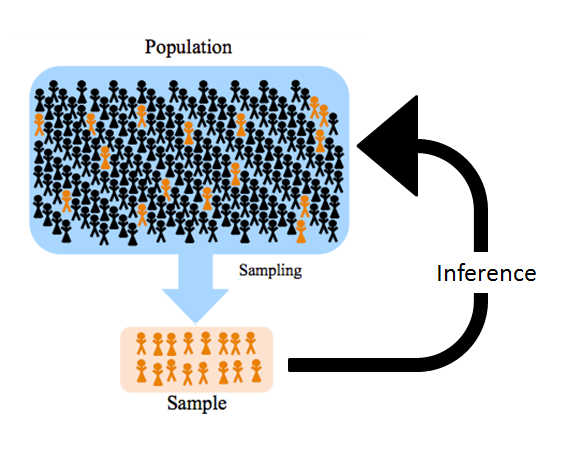
\includegraphics[width=0.6\textwidth]{stats_img/population_sample.png}
		\source{\url{https://online.stat.psu.edu/stat500/}}
	\end{figure}
\end{frame}

% Slide-n
\begin{frame}[t]{Types of Sampling Methods}
	To draw valid conclusions from your results, you have to carefully decide 
	how you will select a sample that is representative of the group as a 
	whole. There are two types of sampling methods
	\begin{itemize}
		\item Probability Sampling
		\item Non-Probability Sampling 
	\end{itemize}
\end{frame}

% Slide-n
\begin{frame}[t]{Probability Sampling Methods}
	\begin{itemize}
		\item Probability sampling involves 
		random selection, allowing you to make statistical inferences about the 
		whole group.
		\item Probability sampling means that every member of the population 
		has a chance of being selected.
		\item It is mainly used in quantitative research.
		\item If you want to produce results that are representative of the 
		whole population, you need to use a probability sampling technique.
	\end{itemize}
\end{frame}

% Slide-n
\begin{frame}[t]{Non-Probability Sampling Methods}
	\begin{itemize}
		\item Non-probability sampling involves 
		non-random selection based on convenience or other criteria, allowing 
		you to easily collect initial data.
	\end{itemize}
\end{frame}

% Slide-n
\begin{frame}[t]{Types of Probability Sampling Methods}
	\begin{figure} [ht]
		\centering
		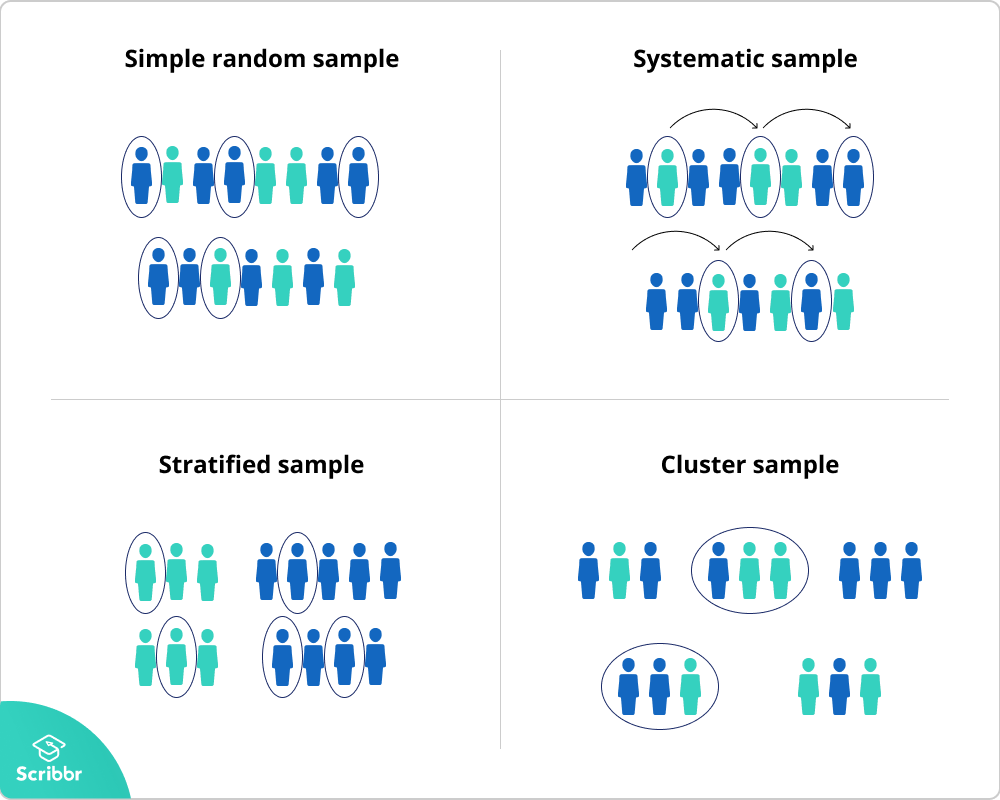
\includegraphics[width=0.6\textwidth]{rp/sampling.png}
		\source{\url{https://www.scribbr.com/methodology/sampling-methods/}}
	\end{figure}
\end{frame}


% Slide-n
\begin{frame}[t]{Simple Random Sampling(SRS)}
	\begin{itemize}
		\item In a simple random sample, every member of the population has an 
		equal chance of being selected. Your sampling frame should include the 
		whole population.
		\item To conduct this type of sampling, you can use tools like random 
		number generators or other techniques that are based entirely on chance.
	\end{itemize}
\end{frame}
% Slide-n
\begin{frame}[t]{Systematic Sampling}
	\begin{itemize}
		\item Systematic sampling is similar to simple random sampling, but it 
		is usually slightly easier to conduct.
		\item Every member of the population is listed with a number, but 
		instead of randomly generating numbers, individuals are chosen at 
		regular intervals.
	\end{itemize}
\end{frame}

% Slide-n
\begin{frame}[t]{ Stratified Sampling}
	\begin{itemize}
		\item Stratified sampling involves dividing the population into 
		subpopulations that may differ in important ways. It allows you draw 
		more precise conclusions by ensuring that every subgroup is properly 
		represented in the sample.
		\item To use this sampling method, you divide the population into 
		subgroups (called strata) based on the relevant characteristic (e.g. 
		gender, age range, income bracket, job role).
		\item Based on the overall proportions of the population, you calculate 
		how many people should be sampled from each subgroup. Then you use 
		random or systematic sampling to select a sample from each subgroup.
	\end{itemize}
\end{frame}

% Slide-n
\begin{frame}[t]{Cluster Sampling}
	\begin{itemize}
		\item Cluster sampling also involves dividing the population into 
		subgroups, but each subgroup should have similar characteristics to the 
		whole sample. Instead of sampling individuals from each subgroup, you 
		randomly select entire subgroups.
		\item If it is practically possible, you might include every individual 
		from each sampled cluster. If the clusters themselves are large, you 
		can also sample individuals from within each cluster using one of the 
		techniques above.
		\item This method is good for dealing with large and dispersed 
		populations, but there is more risk of error in the sample, as there 
		could be substantial differences between clusters. It’s difficult to 
		guarantee that the sampled clusters are really representative of the 
		whole population.
	\end{itemize}
\end{frame}


\begin{frame}[t]{Data Collection Methods}
	\begin{itemize}
		\item \textbf{Survey:}  Survey research allows you to gather large 
		volumes of 
		data that can be analyzed for frequencies, averages and patterns.
		\item \textbf{Observations:} Observations allow you to gather data on 
		behaviours and phenomena without having to rely on the honesty and 
		accuracy of respondents. This method is often used by psychological, 
		social and market researchers to understand how people act in real-life 
		situations.
		\item \textbf{Case Study:} A case study can be used to describe the 
		characteristics of a specific subject (such as a person, group, event 
		or organization). Instead of gathering a large volume of data to 
		identify patterns across time or location, case studies gather detailed 
		data to identify the characteristics of a narrowly defined subject.
		
		\item Interviews 
		\item Experiment 
	\end{itemize}
\end{frame}





% Slide-n
\begin{frame}[t]{Types of Statistical Methods}
	\begin{itemize}
		\item \textbf{Descriptive Statistics:} Identify important elements in a
		dataset.
		\item \textbf{Inferential Statistics:} Explain those elements via
		relationships with other elements.
	\end{itemize}
\end{frame}

% Slide-n
\begin{frame}[t]{Descriptive Statistics}
	Descriptive Statistics divide into 3 categories.
	\begin{itemize}
		\item \textbf{Univariate Analysis:}  summarize only one variable at a 
		time.
		\item \textbf{Bivariate Analysis:}  compare two variables.
		\item \textbf{Multivariate Analysis:}  compare more than two variables.
	\end{itemize}
\end{frame}

% Slide-n
\begin{frame}[t]{Characteristics of Descriptive Statistical Methods}
	\begin{itemize}
		\item Descriptive statistical methods provide an exploratory
		assessment of the data from a study
		\item Exploratory data analysis techniques
		\item Organization and summarization of data
		\begin{itemize}
			\item Tables
			\item Graphs
			\item Summary measures
		\end{itemize}
	\end{itemize}
\end{frame}


\begin{frame}[t]{Inferential Statistics}
	Inferential Statistics divide into 2 categories.
	\begin{itemize}
		\item \textbf{Hypothesis
			Testing:} A hypothesis is a statement that can be tested by 
		scientific research.
		\item \textbf{Model Fitting:} Model fitting is a measure of how well a 
		statistical learning model generalizes to similar data to that on which 
		it was trained.
	\end{itemize}
\end{frame}


% Slide-n
\begin{frame}[t]{Characteristics of Inferential Statistical Methods}
	\begin{itemize}
		\item Assess the strength of evidence for/against a hypothesis.
		\item Inferential statistical methods provide a confirmatory
		data analysis.
		\item Generalize conclusions from data from part of a
		group (sample) to the whole group (population)
		\item Assess the strength of the evidence
		\item Make comparisons.
		\item Make predictions.
		\item Ask more questions; suggest future research.
	\end{itemize}
\end{frame}



% Slide-n
\begin{frame}[t]{Steps in a Research Project}
(1) \fbox{Questions} $\rightarrow$ \fbox{Why?} $\rightarrow$ \fbox{Literature 
Review} $\leftarrow$ \fbox{Iterative Process}

\vspace{20pt}

(2) \fbox{Study Design} $\rightarrow$ \fbox{Study Subject} $\rightarrow$ 
\fbox{Data Collection} $\rightarrow$ \fbox{Dummy Table/Shell Table} 

\vspace{20pt}

(3) \fbox{Statistical Analysis} $\rightarrow$ \fbox{Manuscript} $\rightarrow$ 
\fbox{Publication} 
	
\end{frame}

% Slide-n
\begin{frame}[t]{Planning/ Study Design}
	\begin{itemize}
		\item Primary question(s) of interest
		\begin{itemize}
			\item[--] Quantifying information about a single group?
			\item [--] Comparing multiple groups?
		\end{itemize}
		\item Sample Size 
		\begin{itemize}
			\item[--] How many subjects needed total?
			\item [--] How many in each of the groups to be compared?
		\end{itemize}
	
		\item Selecting study participants
		\begin{itemize}
			\item [--] Randomly chosen from “master list?”
			\item [--]Selected from a pool of interested persons?
		\end{itemize}
	
		\item Sampling Methods 
		\begin{itemize}
			\item [--] Probabilistic methods?
			\item [--] Non-probabilistic methods?
		\end{itemize}
	\end{itemize}
\end{frame}


\begin{frame}[t]{Data Collection}
	First, decide how you will collect data. Your methods depend on what type 
	of data you need to answer your research question. 
	\begin{itemize}
		\item Qualitative or Quantitative?
		\item Primary or Secondary?
		\item Descriptive or Experimental?
	\end{itemize}
\end{frame}


% Slide-n
\begin{frame}[t]{Data Analysis}
	After collecting data, decide how you will analyze the data.
	\begin{itemize}
		\item For quantitative data, you can use statistical analysis methods 
		to test relationships between variables.
		\item For qualitative data, you can use methods such as thematic 
		analysis to interpret patterns and meanings in the data.
	\end{itemize}
\end{frame}


% Slide-n
\begin{frame}[t]{Interpretation}
	What do the results mean in terms of practice, the program,
	the population etc.?
\end{frame}

% Slide-n
\begin{frame}[t]{Reporting/Manuscript Writing}
	\begin{itemize}
		\item What summary measures will best convey the “main messages”
		in the data about the primary (and secondary) research
		questions of interest
		\item How to convey/ rectify uncertainty in estimates based on the
		data
	\end{itemize}
\end{frame}
% Slide-n
\begin{frame}[t]{Publication}
	\vfill
	\centering \LARGE Publish Your Research $\dots$
\end{frame}


% Slide-refs
\begin{frame}[t]{References}
	\begin{itemize}
		\item \url{https://www.formpl.us/blog/research/home}
		\item \url{https://www.scribbr.com/methodology/}
		\item \url{https://www.questionpro.com/blog/}
		\item \url{https://www.scribbr.com/category/research-process/}
		\item 
		\url{https://ocw.jhsph.edu/index.cfm/go/viewCourse/course/FundEpi/coursePage/index/}
	\end{itemize}
\end{frame}

% Thank you slide 
\plain{Thank You\\ \ \\ \Huge{\smiley}}
\end{document}